\cardfrontfoot{Kapitel 19}

\begin{flashcard}[Teori]{Hvad vil det sige at en ligang er mono-, bi-, etc. dentat?}
En monodentat ligand binder ved at donere et lonepair, en bidentat med to, tetradentat med fire osv.. Oxalat ionen er et eksempel på en chelat ligand.
\end{flashcard}

\begin{flashcard}[Struktur]{Tegn strukturen af ethylendiamintetraacetat $(\rm edta)^{4-}$ ionen}
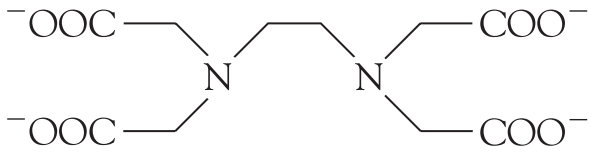
\includegraphics[width=0.8\textwidth]{figures/k19s503edta.png}
\end{flashcard}

\begin{flashcard}[Teori]{Vis med et eksempel hvad der forstås ved \textit{linkage isomerism}}
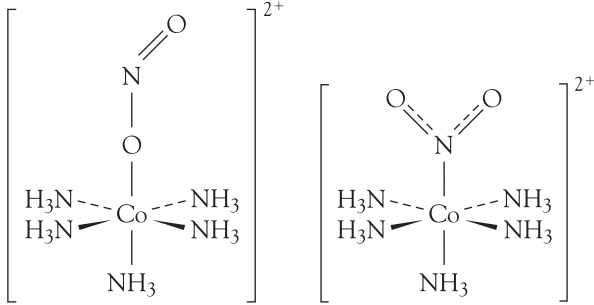
\includegraphics[width=0.8\textwidth]{figures/k19s504linkageisomerism.png}\\\vspace*{0.7cm}
hhv. \ce{[Co(ONO)(NH3)5]^{2+}} og \ce{[Co(NO2)(NH3)5]^{2+}} ionen
\end{flashcard}

\begin{flashcard}[Teori]{\ce{Co(NH3)5Br(SO4)} optræder i flere former. En af disse indeholder \ce{[CoBr(NH3)5]^{2+}} ionen mens en anden indeholder \ce{[CoSO4(NH3)5]^{+}} ionen. Hvilken slags isomeri er dette et eksempel på?}
Ion isomeri
\end{flashcard}

\begin{flashcard}[Teori]{Forklar med et eksempel hvad der forstås ved hydratiseringsisomeri}
Forbindelser der indeholder forskellige mængder krystalvand.
Ex. \ce{CrCl3*6H2O}, \ce{[CrCl(OH2)5]Cl2*H2O} og \ce{[CrCl2(OH2)4]Cl*2H2O}
\end{flashcard}

\begin{flashcard}[Teori]{Vis med et eksempel hvad der forstås ved koordinationsisomeri}
Når en forbindelse bestående af minimum to komplekser bytter ligander hvilket leder til en ny forbindelse. Ex. \ce{[Cr(NH3)6][Co(CN)6]} og \ce{[Co(NH3)6][Co(CN)6]}
\end{flashcard}

\begin{flashcard}[Teori]{Tegn de mulige stereoismere af et plankvadratisk kompleks}
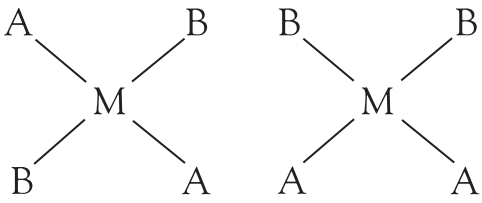
\includegraphics[width=0.8\textwidth]{figures/k19s505kvadisomere.png}
\end{flashcard}

\begin{flashcard}[Teori]{Tegn de mulige stereoismere af et oktaederisk kompleks}
\vspace*{-0.2cm}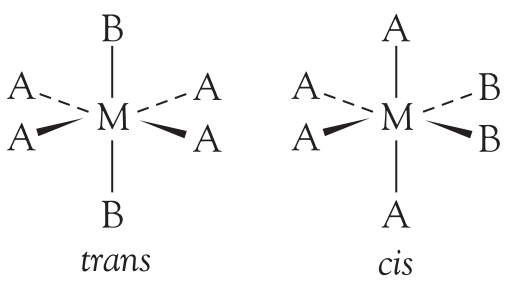
\includegraphics[width=0.5\textwidth]{figures/k19s505hexcistrans.png}\vspace*{0.5cm}
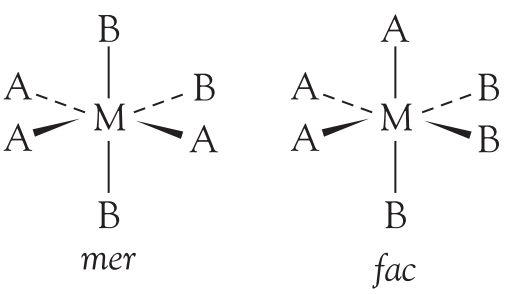
\includegraphics[width=0.5\textwidth]{figures/k19s506hexmerfac.png}
\end{flashcard}

\begin{flashcard}[Teori]{Giv et eksempel på hvordan et chiralt kompleks kan se ud}
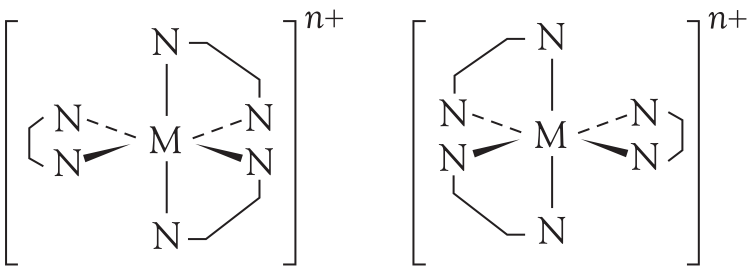
\includegraphics[width=0.9\textwidth]{figures/k19s507chiral.png}
\end{flashcard}



\begin{flashcard}[Teori]{Hvad er den primære begrænsning ved valens bindings teori?}
At teorien ikke kan forudsige men kun rationalisere
\end{flashcard}


\begin{flashcard}[Teori]{Hvilke antagelser gøres i krystalfeltteorien?}
Overgangsmetalionen er fri og på gasform.\\
Liganderne opfører sig som punktladninger.\\
Ingen interaktion mellem metallets $d$ orbitaler og ligandernes orbitaler.
\end{flashcard}


\begin{flashcard}[Teori]{Hvad er drivkraften for kompleksdannelse ifølge CFT?}
En fri gasformig metalions $d$ orbitaler har alle samme energiniveau (degenererede). Når liganderne binder aftager nogle af orbitalerne i energi mens andre vokser. Elektronerne fyldes i de nye lavere energiniveauer hvilket er energetisk favorabelt.
\end{flashcard}


\begin{flashcard}[Teori]{Hvad forstås ved CFSE?}
\textit{crystal felts stabilisations energi}. Den energi der udløses når elektroner går fra degerenrerede $d$ orbitaler til opsplittede $d$ orbitaler.
\end{flashcard}


\begin{flashcard}[Teori]{Hvad er sammenhængene mellem spin, felt og CFSE?}
Høj CFSE svarer til lavt spin hvilket svarer til et stærkt felt.
\end{flashcard}


\begin{flashcard}[Teori]{Hvilke faktorer har indflydelse på CFSE?}
Jo højere periode des højere CFSE.
Jo højere oxidationstrin des højere CFSE.
Jo flere ligander des højere CFSE.
Selve liganderne jvf. den spektrokemiske serie.
\end{flashcard}


\begin{flashcard}[Teori]{Opskriv den spektrokemiske serie}
\ce{I-} < \ce{Br-} < \ce{Cl-} < \ce{F-}\\< \ce{OH-} < \ce{OH2} < \ce{NH3} < \ce{en} < \ce{CN-} < \ce{CO}
\end{flashcard}


\begin{flashcard}[Teori]{Angiv hvorledes elektronerne fordeles i et oktaederiske kompleks}
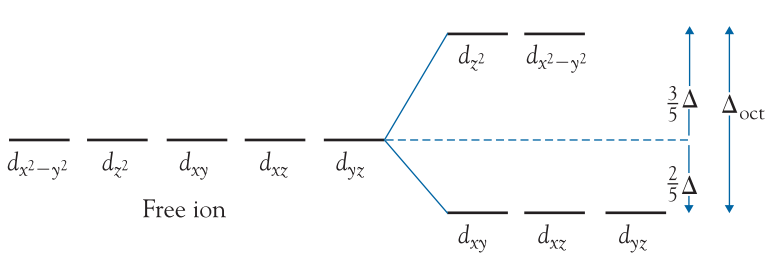
\includegraphics[width=0.9\textwidth]{figures/k19s513mooct.png}
\end{flashcard}


\begin{flashcard}[Teori]{Angiv hvorledes elektronerne fordeles i et tetraederisk kompleks}
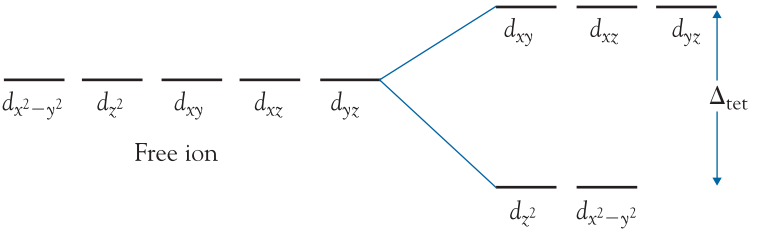
\includegraphics[width=0.9\textwidth]{figures/k19s516motet.png}
\end{flashcard}


\begin{flashcard}[Teori]{Angiv hvorledes elektronerne fordeles i et plankvadratisk kompleks}
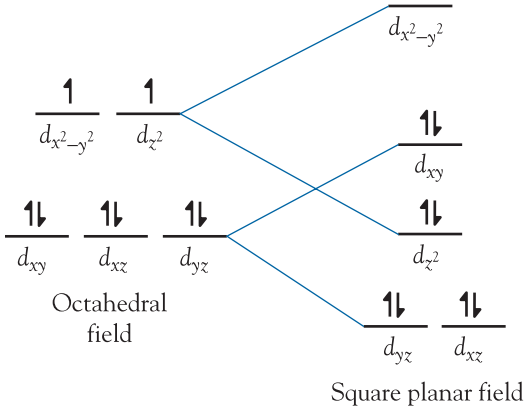
\includegraphics[width=0.8\textwidth]{figures/k19s517mopk.png}
\end{flashcard}


\begin{flashcard}[Teori]{Hvilken farve vil et kompleks have hvis det absorberer i den grønne del af det synlige spektrum?}
Det lys der ikke absorberes reflekteres. Derfor vil den reflektere en blanding af rød og blå dvs. lilla.
\end{flashcard}


\begin{flashcard}[Teori]{Hvilken farve vil du forvente et kompleks har hvis det har en høj CFSE?}
En farve der korresponderer til en kort bølgelængde hvilket svarer til energirig elektromagnetisk stråling. Eksempelvis faverne blå og violet.
\end{flashcard}


\begin{flashcard}[Egenskab]{Hvilke struktur har \ce{MgAl2O4}, \ce{Fe3O4}, \ce{Mn3O4} og \ce{MFe2O4} hvor M er dipositive overgangsmetalioner?}
Spinel, invers spinel, spinel og spinel.
\end{flashcard}


\begin{flashcard}[Teori]{Hvilke komplekser har oftest intense farver?}
Tetraederiske komplekser da de ikke har et symmetripunkt.
\end{flashcard}


\begin{flashcard}[Egenskab]{Forklar hvorfor permangernationen har en stærk farve}
Selvom ionen har en $d^{0}$ konfiguration kan der stadig ske elektronovergange via charge transfer fra oxygenatomets $p$ orbitaler til mangans ledige $d$ orbitaler.
\end{flashcard}


\begin{flashcard}[Teori]{Hvad forstås ved spinforbudte henholdsvis laporte forbudte elektronovergange?}
Spin: Sandsynligheden for ændring af spin er meget lille.\\
Laporte: Overgange mellem $d$ orbitaler er forbudte når molekylet har et inversionscenter.
\end{flashcard}


\begin{flashcard}[Egenskab]{Hvorfor er \ce{Cr^{3+}} og \ce{Co^{3+}} komplekser ofte inerte?}
De har 3 henholdsvis 6 $d$ elektroner i grundtilstanden. Med en oktaederisk konfiguration er de halvfyldte henholdsvis fyldte laveste $d$ energiniveauer så stabile at der ikke er aktiveringsenergien bliver høj.
\end{flashcard}


\begin{flashcard}[Teori]{Nævn tre typer af reaktioner til syntese af koordinationskomplekser og giv eksempler på dem}
Ligandudskiftning: \ce{[Ni(OH2)6]^{2+} + 6NH3 -> [Ni(NH3)6]^{2+} + 6H2O}\\\vspace*{0.5cm}
Redox:\\\ce{Os + 3F2 -> OsF6}\\\vspace*{0.5cm}
Partiel dekomponering: \ce{[Co(NH3)5(OH2)]Cl3 ->[\text{$\Delta$}] [Co(NH3)5Cl]Cl2 + H2O}
\end{flashcard}


\begin{flashcard}[Fremstilling]{Giv reaktionerne til fremstilling af bariumferrat(IV)}
\ce{2Fe^{3+} + 3ClO- + 10OH- -> 2FeO4^{2-} + 3Cl- + 5H2O}\\\vspace*{0.5cm}
\ce{FeO4^{2-} + Ba^{2+} -> BaFeO4(s)}
\end{flashcard}

\begin{flashcard}[Teori]{Hvad er grundprincippet i HSAB teori?
Angiv også 7 hårde, 2 mellem og 3 bløde ligandatomer}
Hårde ligander binder bedst til hårde overgangsmetaller.
Alle overgangsmetalioner med en ladning over +2 samt \ce{Mn^{+2}} er hårde, dem med +2 er mellem og alle med lavere ladning er bløde.\\\vspace*{0.3cm}
Bløde: \ce{C}, \ce{S}, \ce{As}, \ce{Se}, \ce{Te}, \ce{I}.\\
Mellem: \ce{Cl}, \ce{Br}.\\
Hårde: \ce{N}, \ce{O}, \ce{F}.  
\end{flashcard}


\begin{flashcard}[Teori]{Forklar begrebet \textit{kemisk symbiose}}
Et kompleks med bløde ligander har større tendens til at binde til en blød ligand mere end til at binde til en hård ligand og dermed opnå en "blanding".
Eksempelvis er \ce{[Co(NH3)5F]^{2+}} mere stabil end \ce{[Co(NH3)5I]^{2+}}
\end{flashcard}


\begin{flashcard}[Struktur]{Tegn strukturen af metalloporphyrinkomplekset}
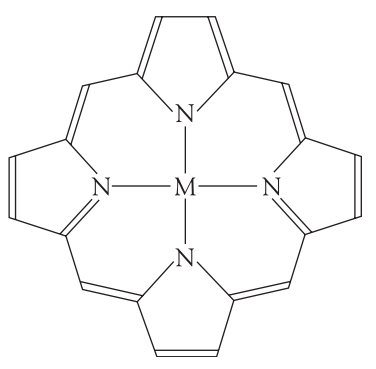
\includegraphics[width=0.6\textwidth]{figures/k19s529porphyrin.png}
\end{flashcard}